\subsection{Geometrical Problem}\label{sec:geomprob}
\Fig{mesh} illustrates the first problem~G1, to mesh around a simple 2-D geometry, an ellipse
with axes parallel to the coordinate axes $x$~and~$y$ indicated.
The mesh sketched in \Fig{mesh} has cells which are exaggeratedly large
but it nonetheless illustrates issues which still arise even for meshes which are much
smaller relative to the geometry.
\begin{figure}
\centerline{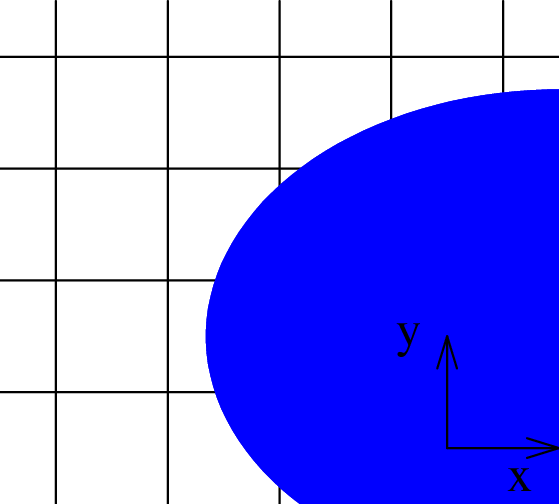
\includegraphics[width=6cm]{../pics/mesh}}
\caption{The G1~problem of meshing round a simple 2-D geometry, an ellipse
with axes parallel to the coordinate axes $x$~and~$y$ indicated.
\label{fig:mesh}}
\end{figure}

\paragraph{Physical Issue}
For example, the ellipse
could represent a specially shaped PFC body, so that numerical solution of a heat
transfer problem is required in the exterior region to determine the temperature
distribution on the elliptical surface. Since it involves edge plasma, a numerical 
discretisation is required which may be either explicit or implicit. In the case
of an explicit scheme, the maximum allowed timestep is given by the time taken for
fluid/plasma to flow across the smallest cell. Implicit schemes are less constrained, but
generally have better convergence properties if cell sizes vary smoothly across
the domain of interest.

A second geometry~G2 is illustrated in \Fig{gaps}. This could be a significant extension of 
a larger volume extruded to model heat transfer by plasma in the gaps between the first wall
tiles. Thus numerical calculation is needed only in the area which is shown white in the figure,
which is shown exaggeratedly large compared to the relative inter-tile spacing in most devices.
\begin{figure}
\centerline{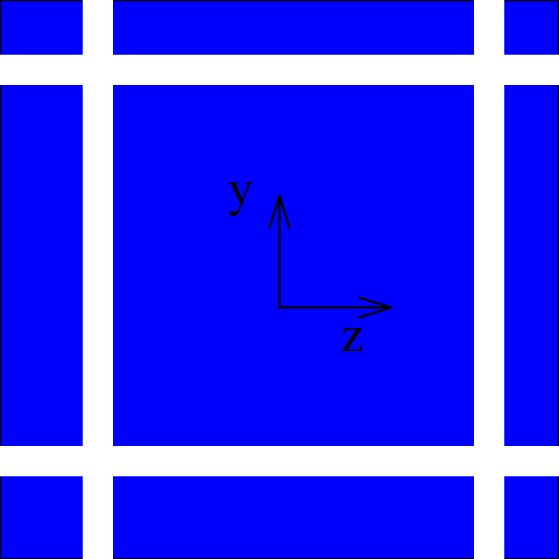
\includegraphics[width=6cm]{../pics/gaps}
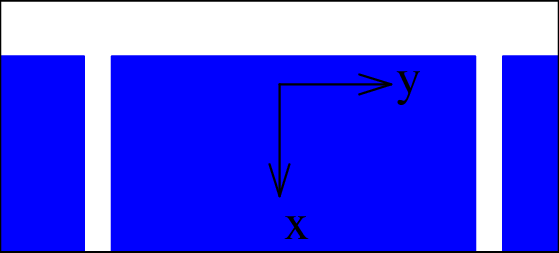
\includegraphics[width=6cm]{../pics/vgaps}
}
\caption{The G2~problem of meshing in the gaps between solid bodies, bodies shown in blue.
The sketch at
right shows a typical slice in a vertical plane aligned with either the $y$ or $z$~axis,
showing a shallow connecting volume above the bodies.
\label{fig:gaps}}
\end{figure}

\clearpage
\subsection{Cell masking}\label{sec:mask}
For G1, the first approach that might be considered is to identify cells within the surface
geometry and exclude them from the modelling. The natural metric for deciding where
a cell lies is the fraction of body it contains. Taking $0.5$ as the cut-off
gives rise to the pixellated G1~geometry of \Fig{mellpix} which will be seen
has one obvious difficulty, namely
deciding what should be taken as the surface normal.
\begin{figure}
\centerline{\includegraphics[width=6cm]{../pics/mellpix}}
\caption{Pixellated mesh geometry. The dashed line represents the original ellipse boundary.
\label{fig:mellpix}}
\end{figure}

Note that masking already gives rise to a need to consider meshing as a separate issue,
in that finite-difference cells have to separated into three separate categories depending on whether
they lie entirely inside, outside or intersect the edges of the bodies.  Moreover for the
last category, the area of cell inside the body has somehow to be computed accurately.

\clearpage
\subsection{Multiblock}\label{sec:multiblock}
Problem~G2 illustrates the fact that there is problem with finite difference
meshes even when the geometry has a simple rectilinear form, in that \Fig{gaps}
indicates that, assuming a uniform grid spacing, most of the cells will be inactive.
This leads to the multiblock approach illustrated in \Fig{vgapp}, where the mesh is
confined to the white areas surrounded by thick black lines. The problem is that
although each block is cuboidal and might be treated using finite differences in its
interior, there are potential issues at the joins, and the need for a complex data
structure to describe how they interconnect.
\begin{figure}
\centerline{\includegraphics[width=6cm]{../pics/vgapp}}
\caption{The heavy lines indicate possible multiblock boundaries in a vertical plane
for the G2~geometry.
\label{fig:vgapp}}
\end{figure}

\clearpage
\subsection{Mesh refinement}\label{sec:meshref}
\subsubsection{Finite difference mesh refinement}\label{sec:fdmeshref}
In problem~G1, clearly some form of mesh refinement near the boundary is required. \Fig{dmesh} shows
a close-up of the region near the `nose' of the ellipse, and \Fig{fd} indicates what happens
if the mesh is refined by insertion of extra cells. To preserve the simple $(x,y)$ addressing
structure, it is necessary to insert entire row or columns, even though only a few cells
in a particular column may need refinement. If the scheme is explicit however, this extra
cost is dominated by the fact that since there are cell edges that are one-eighth the
original length, $8$~times as many timesteps are needed to model the same elapsed physical time.
\begin{figure}
\centerline{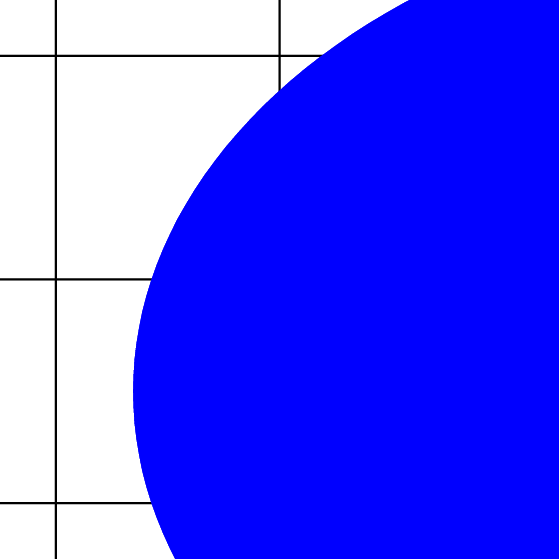
\includegraphics[width=6cm]{../pics/dmesh}}
\caption{Close-up of the G1~problem of meshing round a simple 2-D geometry, an ellipse
with axes parallel to the coordinate axes.
\label{fig:dmesh}}
\end{figure}
\begin{figure}
\centerline{\includegraphics[width=6cm]{../pics/fd}}
\caption{Refinement of finite difference mesh in the G1~problem.
\label{fig:fd}}
\end{figure}

\subsubsection{Hierarchical refinement}\label{sec:hieref}
Another idea is make the cell subdivisions suggested by \Fig{fd} locally. This is illustrated 
in \Fig{mfenabc}. The immediate point to make is that this is \emph{not} a finite-difference mesh, and
addressing the cells shown at right, even though they are each square, will require a
matching hierarchical structure. The problem is worse however because of the so-called
hanging nodes, which occur where larger cells are adjacent to smaller ones, that
require special replacement of the simple finite-difference formulae.
\begin{figure}
\centerline{\includegraphics[width=6cm]{../pics/meshabc}
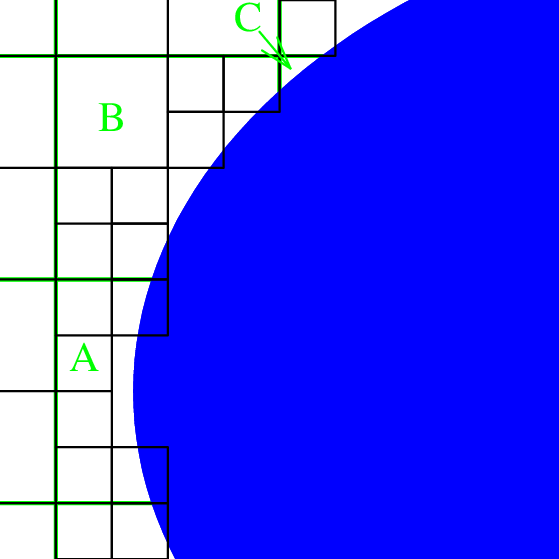
\includegraphics[width=6cm]{../pics/mfenabc}
}
\caption{Close up at right of the cells labelled $A$, $B$ and~$C$ at left, showing
a hierarchy of local refinements by a factor~half. Note that refinements by smaller
factors may be excluded by dividing the larger cell with common boundary,
as indicated.
\label{fig:mfenabc}}
\end{figure}

\clearpage
\subsection{Mapped meshing}\label{sec:mapped}
\begin{figure}
\centerline{\includegraphics[width=6cm]{../pics/basic}
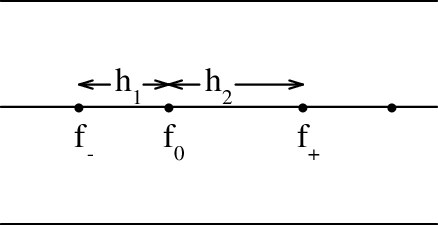
\includegraphics[width=6cm]{../pics/basic2}
}
\caption{A 1-D mapping takes points separated by~$h$ to non-equispaced separation.
\label{fig:basic}}
\end{figure}
With reference to \Fig{basic}(right),
recall the usual approach to deriving finite difference approximation by
means of Taylor series
\begin{eqnarray} \label{eq:taylor}
f_+&=&f_0 + h_2 f'_0 + \frac{1}{2} h_2^2 f^{''}_0 + \frac{1}{6} h_2^3 f^{'''}_0 + \mathcal{O}(h_2^4)\\
f_-&=&f_0 - h_1 f'_0 + \frac{1}{2} h_1^2 f^{''}_0 - \frac{1}{6} h_1^3 f^{'''}_0 + \mathcal{O}(h_1^4)
\end{eqnarray}
Evidently, if $f_0$ and $f_\pm$ are known, then forming the combination 
$h_2 f_- + h_1 f_+ - 2f_0$ eliminates the terms in~$f'_0$ from \Eq{taylor}
to give an approximation $\propto f^{''}_0$,
on rescaling by~$h_1 h_2 \bar{h}$ precisely
\begin{equation} \label{eq:ddf}
f^{''}_0 = \frac{f_-}{h_1 \bar{h}} +  \frac{f_+}{h_2 \bar{h}} -2 \frac{f_0}{h_1 h_2} + \frac{(h_1^2-h_2^2)}{6\bar{h}} f^{'''}_0 + \mathcal{O}(h_1^2,h_2^2)
\end{equation}
where $\bar{h} = (h_1+h_2)/2$. On the uniform grid show at left of \Fig{basic}
where $h_1=h_2=h$, the coefficient of the~$f^{'''}_0$
term vanishes, and the finite-difference approximation is second order, but otherwise unless $h_1\approx h_2$
an order of accuracy is lost. 
One or more orders of loss of accuracy turns out to be a general feature of mapped
finite difference meshes.  Fletcher % ~\cite[\S\,12.2.3]{fletcher}, who 
has shown production of an approximation to the second derivative
which is actually inconsistent unless $h_1\approx h_2$.
This is apparently linked to the subtlety that the size of
the error may be \emph{worse} if the mapping is treated as smoother than the finite-difference approximation.

\clearpage
\subsection{Cut cells}\label{sec:cutcells}
The idea here is to replace the curved edges of the G1~body with straight lines within
a cell. There is a variant where the straight lines are forced to be parallel to one
or other coordinate, but \Fig{meshd2} shows the situation where this constraint is
not enforced. An immediate issue is that when the body is convex as here, this approach
systematically underestimates its size, which in some situations means the entire
calculation may correspond to different parameters than originally intended.
The bigger problem is that cells cut in this way are not necessarily $4$-sided,
so that again the finite-difference formulae will need modification. Moreover, a 
cell with very short sides has been introduced, which will have serious
implications for the timestep size of an explicit scheme, and the likely
convergence properties of an implicit one. The number of possible cases to treat
is also potentially exponential in the number of corner nodes as discussed in
the next \Sec{immersed}.
\begin{figure}
\centerline{\includegraphics[width=6cm]{../pics/meshd2} }
\caption{Cut cell approach to approximating geometry, new edges shown as red dashed lines.
\label{fig:meshd2}}
\end{figure}


\clearpage
\subsection{Immersed boundaries}\label{sec:immersed}
This approach is illustrated in \Fig{fdo} for the problem~G1.
Typically a different or modified physical
process is imagined to operate at the nodes just inside the boundary, eg.\ 
in exterior flow problems a large viscous term to damp motion.
One issue that makes these difficult to use in 3-D is that the number
of possible combinations of corner nodes that are separated by the
object boundary is approximately~$2^{N_{cn}}$ where the number of corner
nodes~$N_{cn}=8$ for a cuboid
or other hexahedron. (Obviously the need to treat~$256$ different cases can be reduced
by using rotations to transform to a smaller number of cannonical arrangements,
but this coding is relatively tricky.)
Another big issue is the abrupt change in the effective physics which
can make for slow convergence of implicit problems.
\begin{figure}
\centerline{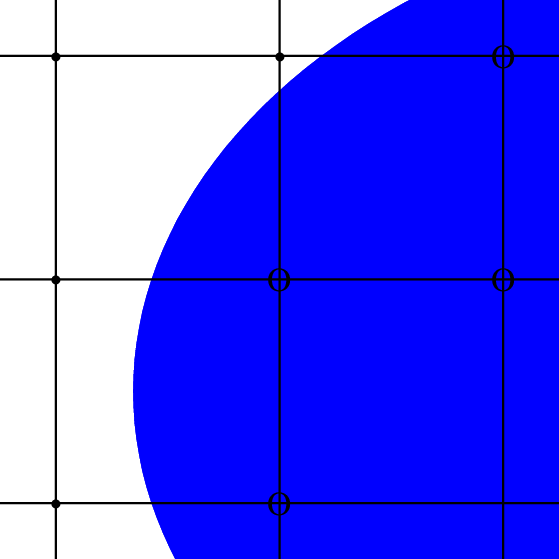
\includegraphics[width=6cm]{../pics/fdo} }
\caption{Immersive approach to boundaries. Cells with open circles at one or more
of their corners have specially modified physics and/or numerics to represent
the fact they intersect the boundary of the body.
\label{fig:fdo}}
\end{figure}

\clearpage
\subsection{Towards Finite Elements}\label{sec:elements}
\Fig{melde} shows how the $5$-sided cells can be eliminated by splitting, and in
this case a small cell eliminated, to give a grid composed mostly of quadrilaterals with 
a few triangles.
(In practice, a further demand would be made on the mesher so that the grid-point
shown as just off the body would be moved onto its surface.) Evidently an implicit scheme
should be used because there remain edges which are relatively short. A yet more
sophisticated mesher could be used to give a more uniform distribution of only
quadrilateral cells in the exterior. This would constitute a good finite element mesh\ldots
\begin{figure}
\centerline{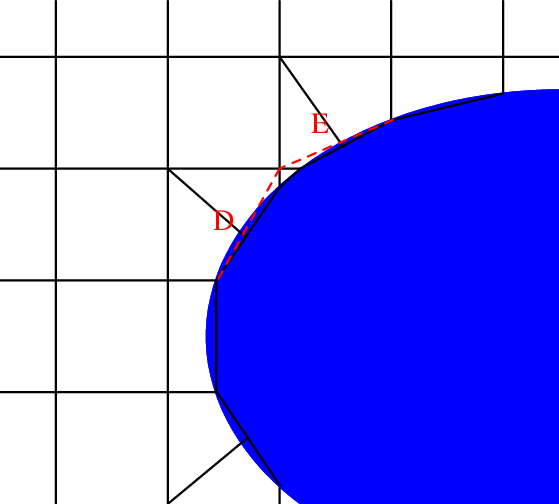
\includegraphics[width=6cm]{../pics/melde} }
\caption{Towards finite elements, all cells are now $4$-sided and mesher
has eliminated very small cell.
\label{fig:melde}}
\end{figure}
%\begin{equation} \label{eq:EQ}
%{\bf v}^T {\bf b} = {\bf v}^T A {\bf x} = (A^T {\bf v})^T {\bf x} = {\bf g}^T {\bf x}
%\end{equation}
